\documentclass[journal=asbcd6,manuscript=article]{achemso}

\usepackage{natbib}
\usepackage{setspace}
\usepackage{xkeyval}
\usepackage{array}
\usepackage{listings}
\usepackage{lmodern}
\usepackage{mathpazo}
\usepackage{geometry}
\usepackage{microtype}
\usepackage{url}  % Formatting web addresses
\usepackage{ifthen}  % Conditional
\usepackage{multicol}   %Columns
\usepackage[utf8]{inputenc} %unicode support
\usepackage{amsmath}
\usepackage{amssymb}
\usepackage{mathtools}
\usepackage{epsfig}
\usepackage{epstopdf}
\usepackage{graphicx}
\usepackage{textcomp}
\usepackage{multirow}
\usepackage{booktabs}
\usepackage{natmove}
\usepackage{float}
\usepackage[margin=0.1pt,font=footnotesize,labelfont=bf]{caption}
\usepackage[version=3]{mhchem} % Formula subscripts using \ce{}
\usepackage[T1]{fontenc}       % Use modern font encodings
%\usepackage[square,sort,comma,numbers,sort&compress]{natbib}
%%%%%%%%%%%%%%%%%%%%%%%%%%%%%%%%%%%%%%%%%%%%%%%%%%%%%%%%%%%%%%%%%%%%%
%% If issues arise when submitting your manuscript, you may want to
%% un-comment the next line.  This provides information on the
%% version of every file you have used.
%%%%%%%%%%%%%%%%%%%%%%%%%%%%%%%%%%%%%%%%%%%%%%%%%%%%%%%%%%%%%%%%%%%%%
%%\listfiles

%\bibliographystyle{achemso}
\newcommand*\mycommand[1]{\texttt{\emph{#1}}}
%%%%%%%%%%%%%%%%%%%%%%%%%%%%%%%%%%%%%%%%%%%%%%%%%%%%%%%%%%%%%%%%%%%%%

%%%%%%%%%%%%%%%%%%%%%%%%%%%%%%%%%%%%%%%%%%%%%%%%%%%%%%%%%%%%%%%%%%%%%
\author{Michael Vilkhovoy}
\author{Nicholas Horvath}
\author{Jeffrey D. Varner}
\email{jdv27@cornell.edu}
\phone{+1~(607)~255-4258}
\fax{+1~(607)~255-9166}
\affiliation[Cornell University]
{Robert Frederick Smith School of Chemical and Biomolecular Engineering, Cornell University, Ithaca, NY 14853}
%%%%%%%%%%%%%%%%%%%%%%%%%%%%%%%%%%%%%%%%%%%%%%%%%%%%%%%%%%%%%%%%%%%%%
\title{Sequence Specific Modeling of Cell-Free Protein Synthesis}
%\abbreviations{MV,NH,JDV}
\keywords{Synthetic biology, Constraints based modeling, Biochemical modeling}

\begin{document}

%%%%%%%%%%%%%%%%%%%%%%%%%%%%%%%%%%%%%%%%%%%%%%%%%%%%%%%%%%%%%%%%%%%%%
%% The abstract environment will automatically gobble the contents
%% if an abstract is not used by the target journal.
%%%%%%%%%%%%%%%%%%%%%%%%%%%%%%%%%%%%%%%%%%%%%%%%%%%%%%%%%%%%%%%%%%%%%
\begin{abstract}
In this study, we used sequence specific constraints based modeling to evaluate the performance of synthetic circuits in an \emph{E.~coli} cell-free protein synthesis system.
A core \emph{E.~coli} metabolic model, consisting of glycolysis, pentose phosphate pathway, amino acid biosynthesis and degradation and energy metabolism, was then augmented with sequence specific descriptions of genetic circuits which included mechanistic models of promoter function, transcription and translation.
Thus, unlike other synthetic biology modeling efforts, sequence specific constraints based modeling explicitly couples the transcription and translation of circuit components with the availability of metabolic resources.
Model parameters for transcription and translation were taken from literature, allowing a first principles prediction of circuit performance.
We tested this approach by first simulating T7 induced CAT production and $\sigma_{70}$-induced deGFP expression; we then expanded these studies for a range of different proteins
First principles predictions of circuit performance were consistent with measurements for a variety of cases.
Further, global sensitivity analysis identified the key metabolic processes that controlled circuit performance in terms of productivity and yield.
A sufficient energy supply with oxidative phosphorylation is instrumental for high carbon yields, in addition the translation rate is the next step to optimize for higher productivity and yield.
Taken together, sequence specific constraints based modeling offers a novel means to \emph{a~priori} estimate the performance of cell-free synthetic circuits.
\end{abstract}

%%%%%%%%%%%%%%%%%%%%%%%%%%%%%%%%%%%%%%%%%%%%%%%%%%%%%%%%%%%%%%%%%%%%%
%% Start the main part of the manuscript here.
%%%%%%%%%%%%%%%%%%%%%%%%%%%%%%%%%%%%%%%%%%%%%%%%%%%%%%%%%%%%%%%%%%%%%

\section{Introduction}
Cell free systems offer many advantages for the study, manipulation and modeling of metabolism compared to \textit{in vivo} processes.
Central amongst these advantages is direct access to metabolites and the microbial biosynthetic machinery without the interference of a cell wall.
This allows us to control as well as interrogate the chemical environment while the biosynthetic machinery is operating, potentially at a fine time resolution.
Second, cell-free systems also allow us to study biological processes without the complications associated with cell growth.
Cell-free protein synthesis (CFPS) systems are arguably the most prominent examples of cell-free systems used today \cite{Jewett:2008aa}.
However, CFPS is not new; CFPS in crude \textit{E.~coli} extracts has been used since the 1960s to explore fundamentally important biological mechanisms \cite{MATTHAEI:1961aa,NIRENBERG:1961aa}.
Today, cell-free systems are used in a variety of applications ranging from therapeutic protein production \cite{Lu:2014aa} to synthetic biology \cite{Hodgman:2012aa}.
Interestingly, many of the challenges confronting in-vivo genome-scale kinetic modeling can potentially be overcome in a cell-free system.
For example, there is no complex transcriptional regulation to consider, transient metabolic measurements are easier to obtain, and we no longer have to consider cell growth.
Thus, cell-free operation holds several significant advantages for model development, identification and validation.
Theoretically, genome-scale cell-free kinetic models may be possible for industrially important organisms, such as \textit{E. coli} or \textit{B. subtilis}, if a simple, tractable framework for integrating allosteric regulation with enzyme kinetics can be formulated.

Stoichiometric reconstructions of microbial metabolism popularized by constraint based modeling techniques such as flux balance analysis (FBA) have become standard tools to interrogate biological networks \cite{2012_lewis_palsson_NatRevMicrobio}.
Since the first genome-scale stoichiometric model of \textit{E. coli}, developed by Edwards and Palsson \cite{2000_edwards_palsson_PNAS}, stoichiometric reconstructions of hundreds of organisms, including industrially important prokaryotes such as \textit{E. coli} \cite{Feist:2007aa} or \textit{B. subtilis} \cite{Oh:2007aa}, are now available \cite{2009_feist_palsson_NatRevMicrobio}.
Stoichiometric models rely on a pseudo-steady-state assumption to reduce unidentifiable genome-scale kinetic models to an underdetermined linear algebraic system, which can be solved efficiently even for large systems using linear programming.
Traditionally, stoichiometric models have also neglected explicit descriptions of metabolic regulation and control mechanisms, instead opting to describe the choice of pathways by prescribing an objective function on metabolism.
Interestingly, similar to early cybernetic models, the most common metabolic objective function has been the optimization of biomass formation \cite{2002_ibarra_edwards_palsson_Nat}, although other metabolic objectives have also been estimated \cite{2007_schuetz_sauer_MolSysBio}.
Recent advances in constraint-based modeling have overcome the early shortcomings of the platform, including capturing metabolic regulation and control \cite{2013_hyduke_lewis_palsson_MolBioSys}. Thus, modern constraint-based approaches are extremely useful for the discovery of metabolic engineering strategies and represent the state of the art in metabolic modeling \cite{2013_mccloskey_palsson_feist_MolSysBio, 2012_zomorrodi_maranas_MetaEng}.

In this study, we used sequence specific constraints based modeling to evaluate the performance of synthetic circuits in an \emph{E.~coli} cell-free protein synthesis (CFPS) system.
A core \emph{E.~coli} cell free metabolic model, consisting of 132 metabolites and 281 reactions, was developed from literature \cite{Feist:2007aa}.
This model, which described glycolysis, pentose phosphate pathway, amino acid biosynthesis and degradation and energy metabolism, was then augmented with
sequence specific descriptions of genetic circuits which included mechanistic models of promoter function, transcription and translation.
Thus, sequence specific constraints based modeling explicitly coupled the transcription and translation of circuit components with the availability of metabolic resources.
We tested this approach by first simulating the production of CAT and deGFP under two different promoters. and then expanded this for $\sigma_{70}$-induced deGFP expression at different plasmid concentrations.
First principles predictions of circuit performance were consistent with measurements.
We then investigated the productivity and carbon yield for a range of 8 different proteins for a variety of cases.
From this, higher carbon number proteins typically had lower productivity rates and carbon yields than that of the lower carbon number proteins.
Further, global sensitivity analysis identified the key metabolic processes that controlled circuit performance, showing oxidative phosphorylation is instrumental for maintaining a high carbon yield and the translation rate for productivity.
Taken together, sequence specific constraints based modeling offers a novel means to \emph{a~priori} estimate the performance of cell free synthetic circuits.

\section{Results and discussion}

\subsection{Model Derivation}
The goal of this work was first to construct a modeling framework to describe cell-free protein synthesis systems and to examine its performance in productivity and yield for a protein of interest.
One mathematical framework that has found wide use in modeling metabolism are constraint based models such as flux balance analysis (FBA).
FBA can predict how cells utilize nutrients to produce products by using the biochemical stoichiometry and thermodynamical feasibility under pseudo steady-state conditions.
Traditionally, FBA is used to model \textit{in vivo} processes, however cell-free systems do not have growth associated reactions or transport through the cell membrane.
Thus, to model cell-free metabolism we constructed a cell-free stoichiometric network by removing growth associated reactions from the MG1655 reconstruction \cite{Feist:2007aa}, and incorporating amino acid synthesis and transcription/translation associated reactions \cite{Allen:2003aa} for a protein of interest to be expressed.
The network consisted of 281 reactions and 132 species.
We developed a cell-free sequence specific flux balance analysis (ssFBA) with a detailed promoter model \cite{Moon:2012aa} to examine the performance of CFPS.
We first validated the ssFBA approach by comparing simulated and measured concentrations of two proteins from two different cell-free \textit{E. coli} extract systems.
The first protein, chloramphenicol acetyltransferase (CAT), was produced under a T7 promoter in a glucose/NMP cell-free system \cite{2005_calhoun_BiotechnologyProgress} for a duration of 1 hour under glucose consumption (Fig \ref{fig:CAT_GFP_prod}A).
The second protein, dual emission green fluorescent protein (deGFP), was produced under a P70 promoter in TXTL 2.0 \textit{E. coli} extract for a duration of 8 hours under maltose consumption (Fig \ref{fig:CAT_GFP_prod}B).
The ssFBA simulations predicted the production of both proteins for the duration of both CFPS batch reactions.
Uncertainty in experimental factors such as RNA polymerase, ribosome concentrations, elongation rates or the upper bounds for oxygen and glucose consumption rates did not alter the qualitative performance of the model.
Thus, the metabolic network and molecular description of trancription and translation were consistent with experimental measurements.
\begin{figure}[t!]
\centering
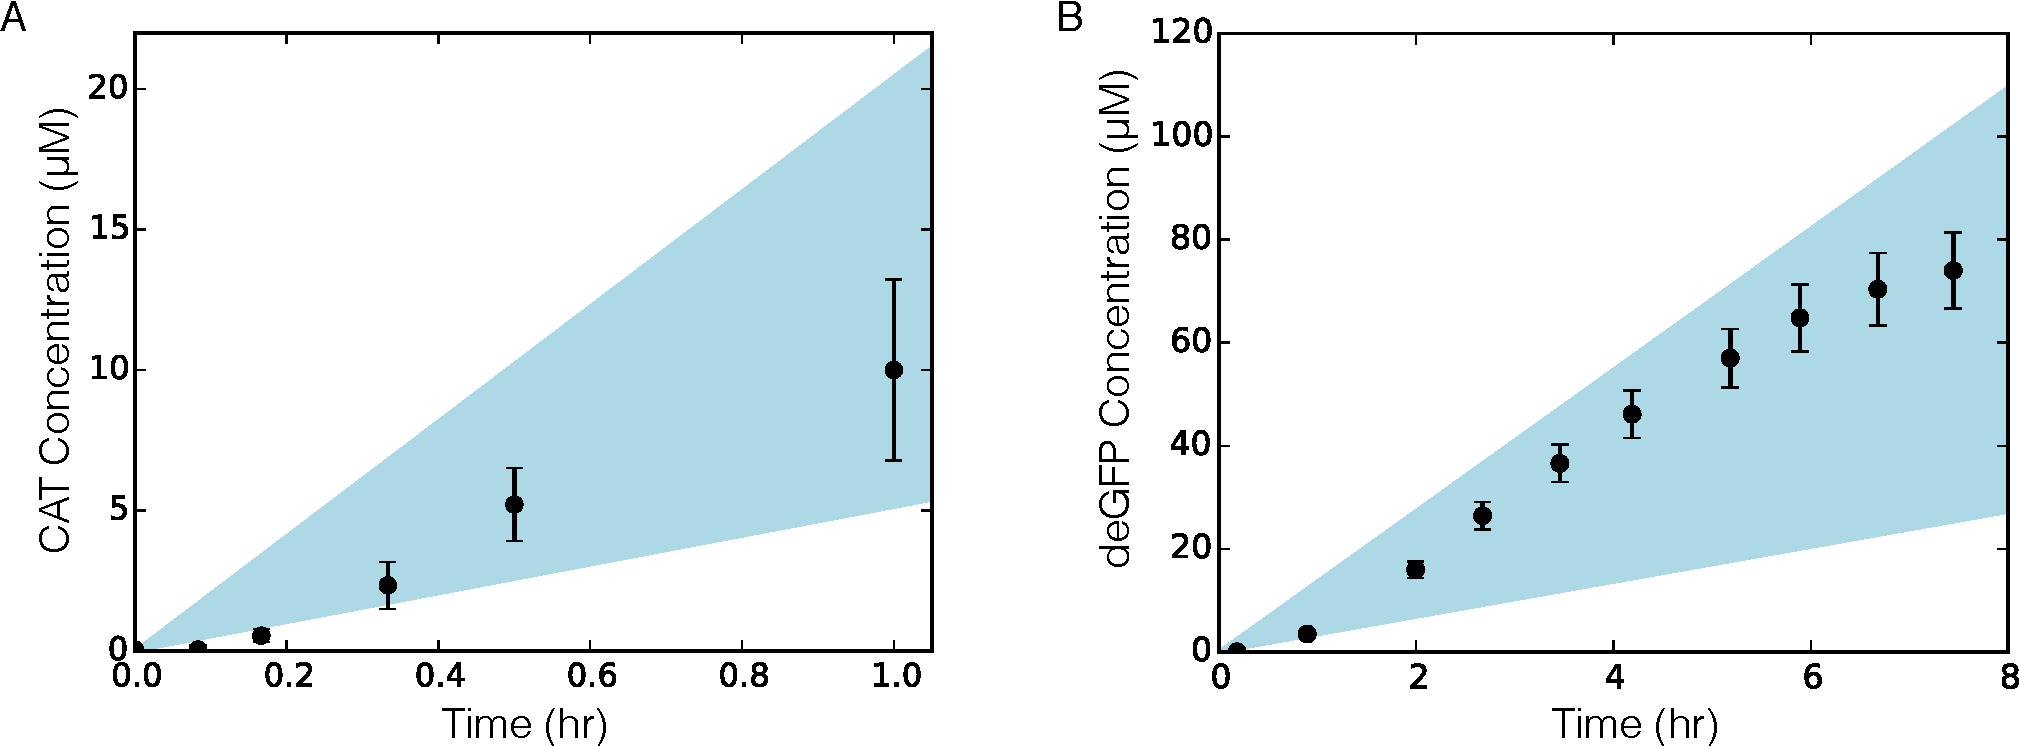
\includegraphics[width=1.00\textwidth]{./Figures/CAT_GFP_prod.pdf}
\caption{Sequence specific flux balance analysis of protein production vesus time. A. CAT production under a T7 promoter in CFPS \textit{E. coli} extract for 1 hr under glucose consumption. B. deGFP production under a P70 promoter in TXTL 2.0 \textit{E. coli} extract for 8 hr under glucose consumption. 95\% CI (blue region) over the ensemble of 100 sets.}
\label{fig:CAT_GFP_prod}
\end{figure}

Next, ssFBA predicted deGFP production as a function of plasmid concentration (Fig \ref{fig:GFP_plasmid}).
Concentration of deGFP at each plasmid concentration was calculated by multiplying the flux of deGFP synthesis by the active time of production, approximately 8 hours in TXTL 2.0 \cite{Garamella:2016aa}.
The mean of the ensemble shows a good prediction against the measured deGFP levels, even though it under predicted deGFP concentration at the saturating point of 5 nM of plasmid concentration.
However, the ensemble and the mean of the ensemble captured the overall saturating dynamics of deGFP production as a function of plasmid concentration.
\begin{figure}[t!]
\centering
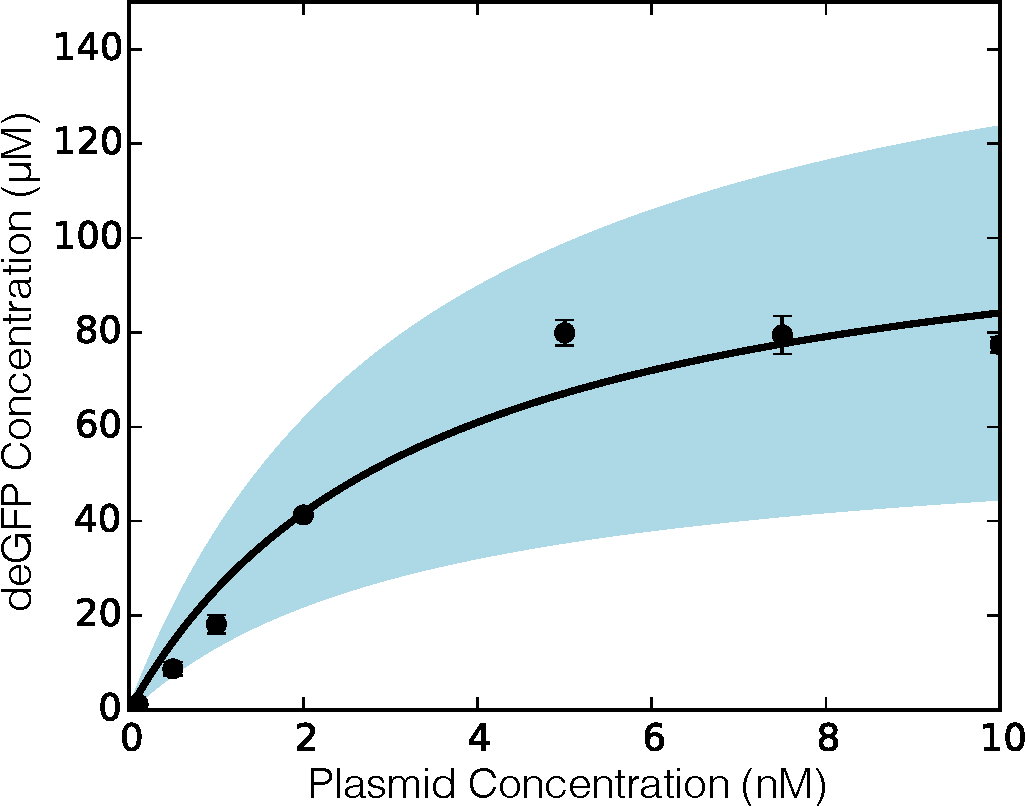
\includegraphics[width=0.6\textwidth]{./Figures/GFP_plasmid.pdf}
\caption{Predicted deGFP concentration (black line) at different plasmid concentrations versus measurements of deGFP (dots) synthesized in TXTL 2.0. 95\% CI (blue region) over the ensemble of 100 sets.}
\label{fig:GFP_plasmid}
\end{figure}

These results validated our mathematical framework to model CFPS systems and predict the production of two proteins with no adjustable parameters.
It also showed that the sequence specific reactions were sufficient to predict the production of two different proteins under two different promoters and cell-free systems.
Since the model accurately predicted the behavior of protein production, we wanted to use our mathematical framework to help us understand the performance limits of CFPS and how these shortcomings could be addressed.

\subsection{CFPS Productivity}
Our next goal was to examine the performance of CFPS productivity for eight different proteins under three different cases. Each of the proteins were produced under a P70 promoter, except for CAT which was produced under a T7 promoter. In all our cases, CFPS is supplied with glucose. The first case, CFPS is supplied with amino acids and the system can synthesize amino acids (control). In the second case, CFPS is supplied with amino acids, however the system cannot synthesize amino acids (AA uptake w/o synthesis). We turned off these synthesis reactions since during the cell-free extract preparation the cells are often supplied with amino acids, thus the enzymes responsible for amino acid synthesis would not be present. In the third case, CFPS is not supplied with amino acids, but the system can synthesize them (AA synthesis w/o uptakte).
Eight different proteins,ranging in size, were selected to evaluate CFPS performance: bone morphogenetic protein 10 (BMP10), chloramphenicol acetyltransferase (CAT), caspase 9 (CASP9), dual emission green fluorescent protein (deGFP), prothrombin (FII), coagulation factor X (FX), fibroblast growth factor 21 (FGF21), and single chain variable fragment R4 (scFvR4).
We used ssFBA to estimate the productivity for each of these proteins for each case (Fig \ref{fig:Prod_POI}A).
The first two cases had very similar performance, with the second case (without amino acid synthesis) having a slightly higher productivity for most proteins. 
%The second case (without amino acid synthesis) showed the highest productivity for each of the proteins, however the control case had very similar performance.
This shows the system had sufficient substrates to power the system and synthesize each protein.
The third case had the lowest productivity for each protein, thus the addition of amino acids to CFPS extract is important for maintaining a relatively high productivity.
The drop in productivity in the third case is due to the fact that glucose is the only substrate supplied and must be used to provide the necessary energy requirements for transcription and translation as well as synthesize each amino acids required for the production of the protein of interest.  
The qualitative trend of productivity for the three different cases was the same within each case, however some proteins had higher productivity than others.
For instance, in the second case FGF21 (fibroblast growth factor 21) had a productivity of 17 ($\mu$M/h) whereas FII (prothrombin) had a productivity of 3 ($\mu$M/h).
To examine this further, the mean productivity was plotted against the carbon number of each protein (Fig \ref{fig:Prod_POI}B).
The proteins with the highest productivity had the lowest carbon number whereas proteins with low productivity had higher carbon numbers.
This inverse qualitative trend was due to the fact that larger proteins require more amino acids and substrates to assemble them resulting in lower productivity.
\begin{figure}[t!]
\centering
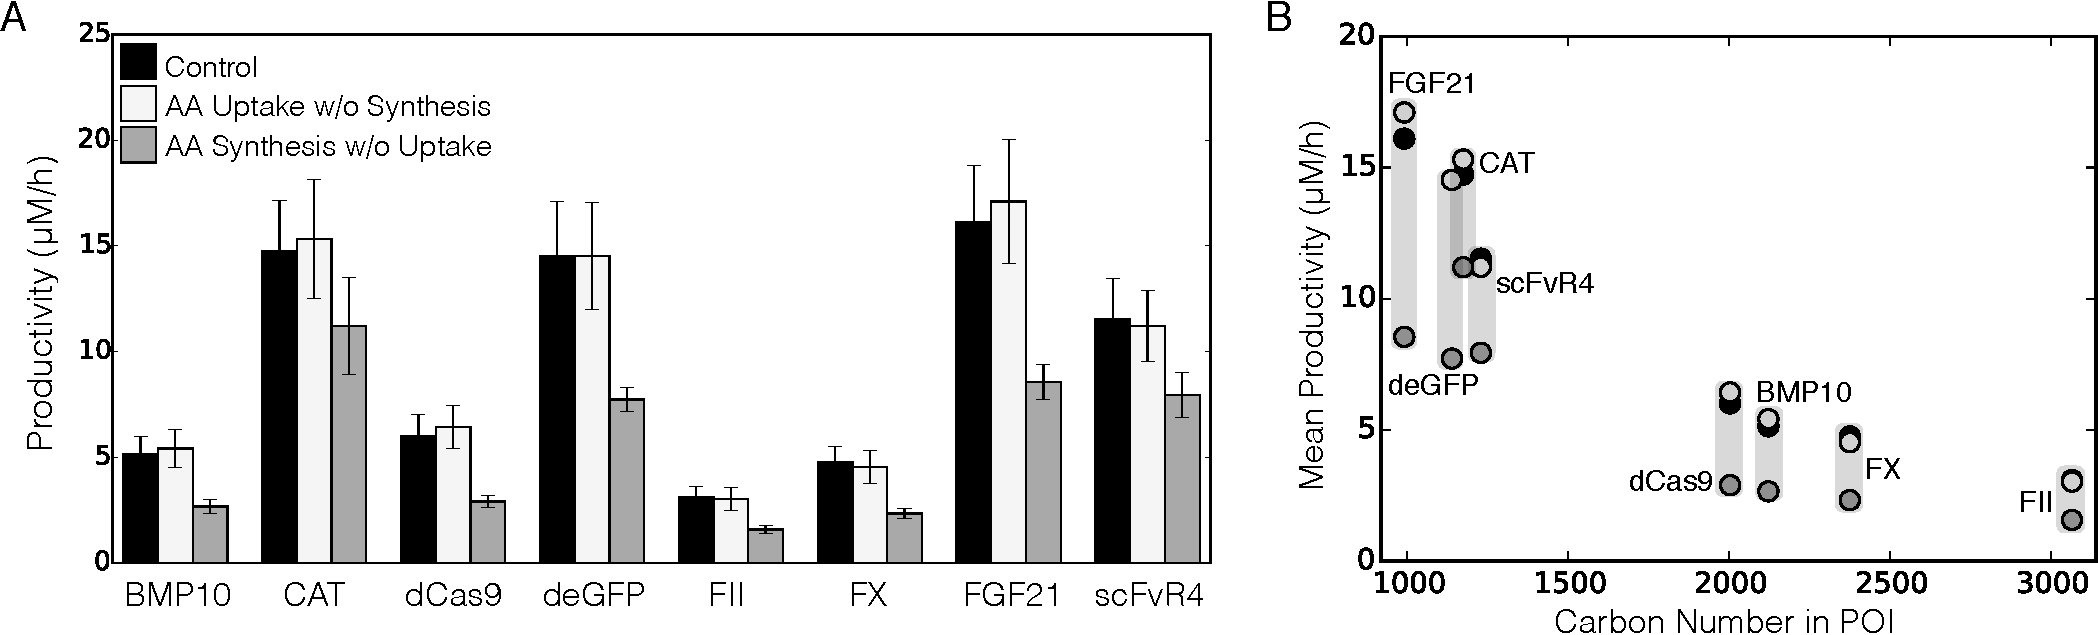
\includegraphics[width=1.00\textwidth]{./Figures/Prod_POI.pdf}
\caption{CFPS productivity performace for eight proteins for the control (black), AA uptake w/o synthesis (off white), and AA synthesis w/o uptake (grey). A. Productivity normalized to the specific glucose uptake rate (Error bars represent the 95\% CI of the ensemble). B. Mean productivity versus the carbon number for each corresponding protein.}
\label{fig:Prod_POI}
\end{figure}

\subsection{CFPS Carbon Yield}
Following the same outline as in examining the productivity, we calculated the carbon yield for each protein (Fig \ref{fig:Yield_POI}A).
The same trends followed, where the case without amino acid synthesis showed the highest carbon yield and the control case had comparable performance.
The third case (with no amino acid uptake) had the lowest yields; this is most likely because glucose is utilized to synthesize the necessary amino acids for each protein as well as power the system. 
To determine the carbon contribution from each substrate (glucose and amino acids) we examined the carbon flux going toward the production of deGFP for all three cases (Table \ref{tbl:yield_breakdown}).
For the first case, the system is relied on a mixture of glucose and some amino acids for the productin of deGFP with a carbon yield of 20.5\%.
Once amino acid synthesis is removed from the network (2nd case), each amino acid is utilized and the carbon yield increased to 22.2\%.
Only the necessary amount of amino acids were used for the production of deGFP, thus it may be hypothesized that all the glucose was used to power CFPS and does not contribute to the carbon yield.
If that is the case, the carbon yield without glucose contribution is 100\%, whereas for the first case its 92.5\%.
Finally for the third case (without amino acid supplemented), the carbon yield was reduced to 14.8\% and the system used about double the amount of glucose as the first two cases.
In this case glucose is being used to synthesize amino acids and provide the necessary energy requirements to power transcription and translation; this trend was seen across all proteins except for CAT.
Interestingly, CAT carbon yield showed similar performance for all three cases, however it still had a lower yield than the first two cases.
Each protein has different energy requirements for transcription and translation depending on its sequence.
Thus, for the case of CAT, energy requirements for transcription or translation were low enough that it's carbon yield was not hindered in the third case as significantly as for the other proteins.

\begin{table}[t!]
\centering
    \caption{Carbon contribution from glucose and each amino acid toward deGFP production for three cases: control, amino acid uptake without synthesis, and amino acid synthesis without uptake.}
    \renewcommand{\arraystretch}{0.9}
    \begin{tabular}{lccc} \toprule
        \parbox{3.2 cm}{Carbon \phantom{abcdefghi} Produced (mM)} & Control & \parbox{2.5 cm}{AA uptake \phantom{ai} w/o synthesis} & \parbox{2.5 cm}{AA synthesis w/o uptake} \\ \midrule
        deGFP & 9.8 & 9.6 & 9.9  \\ \toprule
        \parbox{3.2 cm}{Carbon \phantom{abcdefghi} Consumed (mM)} & \\ \midrule
        GLC & 37.3 & 33.7 & 66.9 \\
        ALA & 0.0 & 0.2 & -  \\
        ARG & 0.3 & 0.3 & - \\
        ASN & 0.5 & 0.4 & -  \\
        ASP & 0.4 & 0.6 & -  \\
        CYS & 0.2 & 0.1 & -  \\
        GLU & 2.1 & 0.6 & -  \\
        GLN & 0.4 & 0.3 & - \\
        GLY & 0.3 & 0.3 & -  \\
        HIS & 0.5 & 0.5 & - \\
        ILE & 0.0 & 0.6 & -  \\
        LEU & 1.0 & 1.0 & - \\
        LYS & 1.0 & 0.9 & - \\
		MET & 0.0 & 0.2 & -  \\
        PHE & 1.0 & 0.9 & - \\
        PRO & 0.4 & 0.4 & -  \\
        SER & 0.0 & 0.2 & - \\
        THR & 1.0 & 0.5 & -  \\
        TRP & 0.1 & 0.1 & -  \\
        TYR & 0.8 & 0.8 & - \\
        VAL & 0.6 & 0.7 & - \\ \hline
        Sum & 47.9 & 43.3 & 66.9  \\ \toprule
        Yield & 20.5\% & 22.2\% & 14.8\% \\
	Yield w/o GLC & 92.5\% & 100\% & - \\ \bottomrule
    \end{tabular}
\label{tbl:yield_breakdown}
\end{table}

We next investigated the effect of the carbon number of each protein to the carbon yield (Fig \ref{fig:Yield_POI}B).
The same inverse qualitative trend is observed as for productivity, however it was less significant.
The proteins with the lowest carbon number had the highest yield and the higher carbon number proteins had a lower carbon yield within each case. 
As the size of the protein to be expressed increases, the productivity and carbon yield decreases, thus proteins that are too large may not be feasible for cell-free production.
Thus, we wanted to examine the most sensitive parameters for cell-free productivity and carbon yield in order to optimize CFPS systems most effectively.
%Sequence specific flux balance analysis assumes a psuedo steady state, thus intermediate metabolites cannot be accumulated within the cell-free extract.
%In addition, ssFBA is solved by setting the production of the protein as the objective function.
%Therefore, carbon flux will travel throughout the network to optimize the flux through the protein synthesis reaction.
\begin{figure}[t!]
\centering
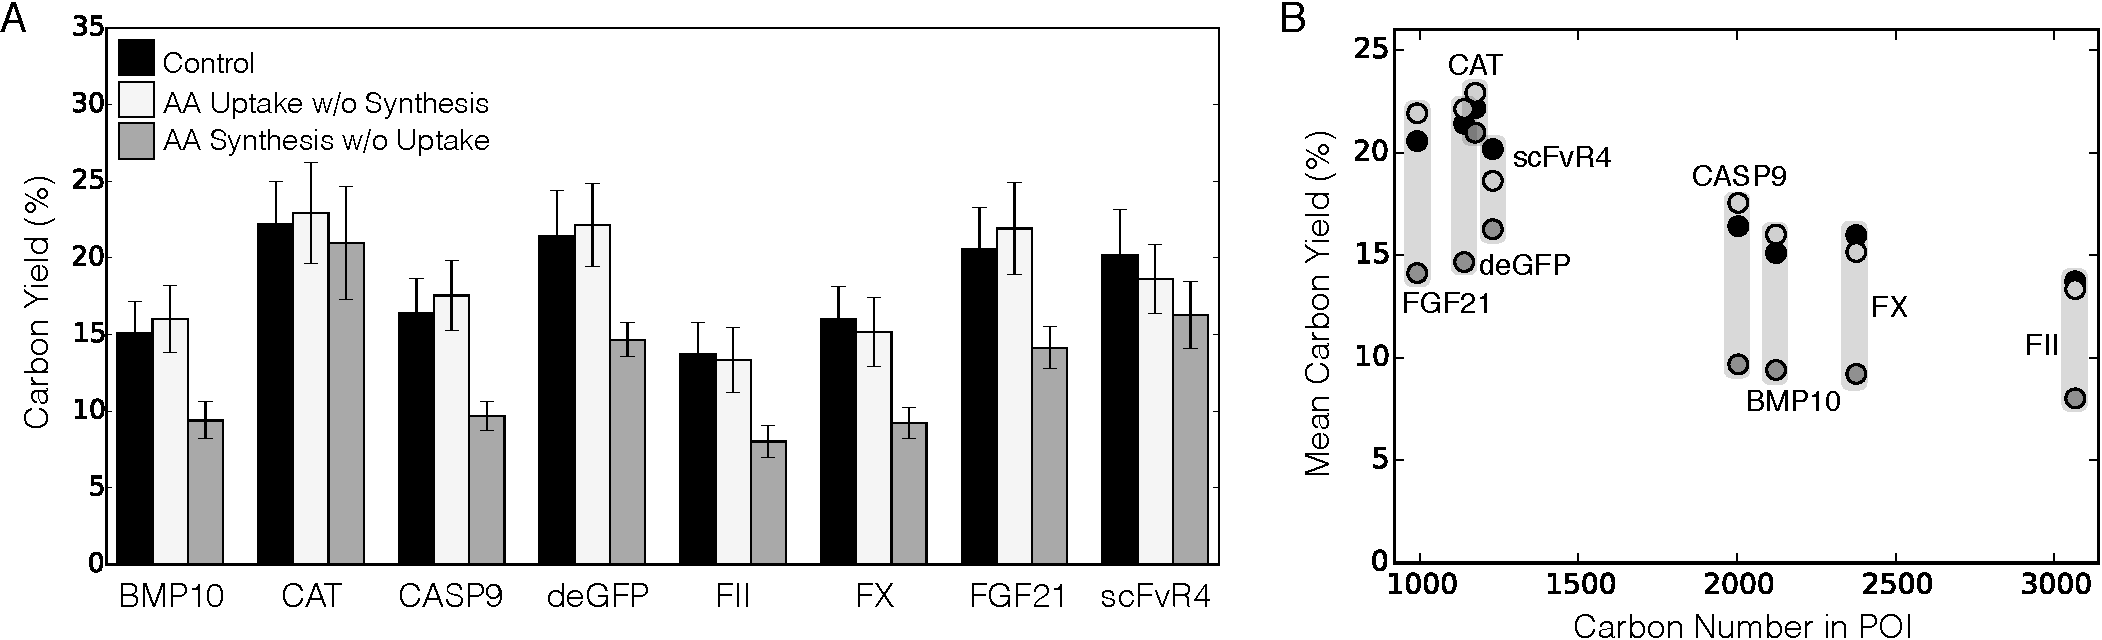
\includegraphics[width=1.00\textwidth]{./Figures/Yield_POI.pdf}
\caption{CFPS carbon yield performace for eight proteins for the control (black), AA uptake w/o synthesis (off white), and AA synthesis w/o uptake (grey). A. Carbon yield (Error bars represent the 95\% CI of the ensemble). B. Mean carbon yield versus the carbon number for each corresponding protein.}
\label{fig:Yield_POI}
\end{figure}


\subsection{CFPS performance sensitivity analysis}
To better understand the effect of substrate utilization and the transcription/translation parameters on CFPS performance we performed global sensitivity analysis on the productivity and carbon yield for deGFP, a representative protein (Fig \ref{fig:SI_GFP}).
In examining productivity performance (Fig \ref{fig:SI_GFP}A), the significance of transcription/translation parameters were fairly constant across all three cases, with the elongation rate by ribosomes being the most sensitive.
This showed the rate of translation is instrumental in achieving high productivity, and should be the first step to investigate in order to optimize productivity, prior to examining transcription rates, this is consistent with literature findings.
Underwood and coworkers have also shown that an increase in ribosome levels does not significantly increase protein yields or rates; however, adding elongation factors increased yields by 23\% at 30 minutes \cite{2005_underwood_biotech}.
In addition, Li et al. have increased productivity of firefly lucifease by 5-fold in CFPS systems by adding and adjusting factors that affect transcription and translation such as elongation factors, ribosome recyclcing factor, release factors, chaperones, BSA, and tRNAs \cite{2014_li_PlosOne}.
In examining the substrate utilization, glucose uptake was not very important for productivity in the first two cases, but its significance increased when amino acids were removed from CFPS.
This makes sense, as amino acid synthesis can only come from glucose and became the only way to power protein synthesis.
On the other hand, when amino acid synthesis is removed, amino acid uptake became more important, as it becomes the only source of amino acids.
\begin{figure}[t!]
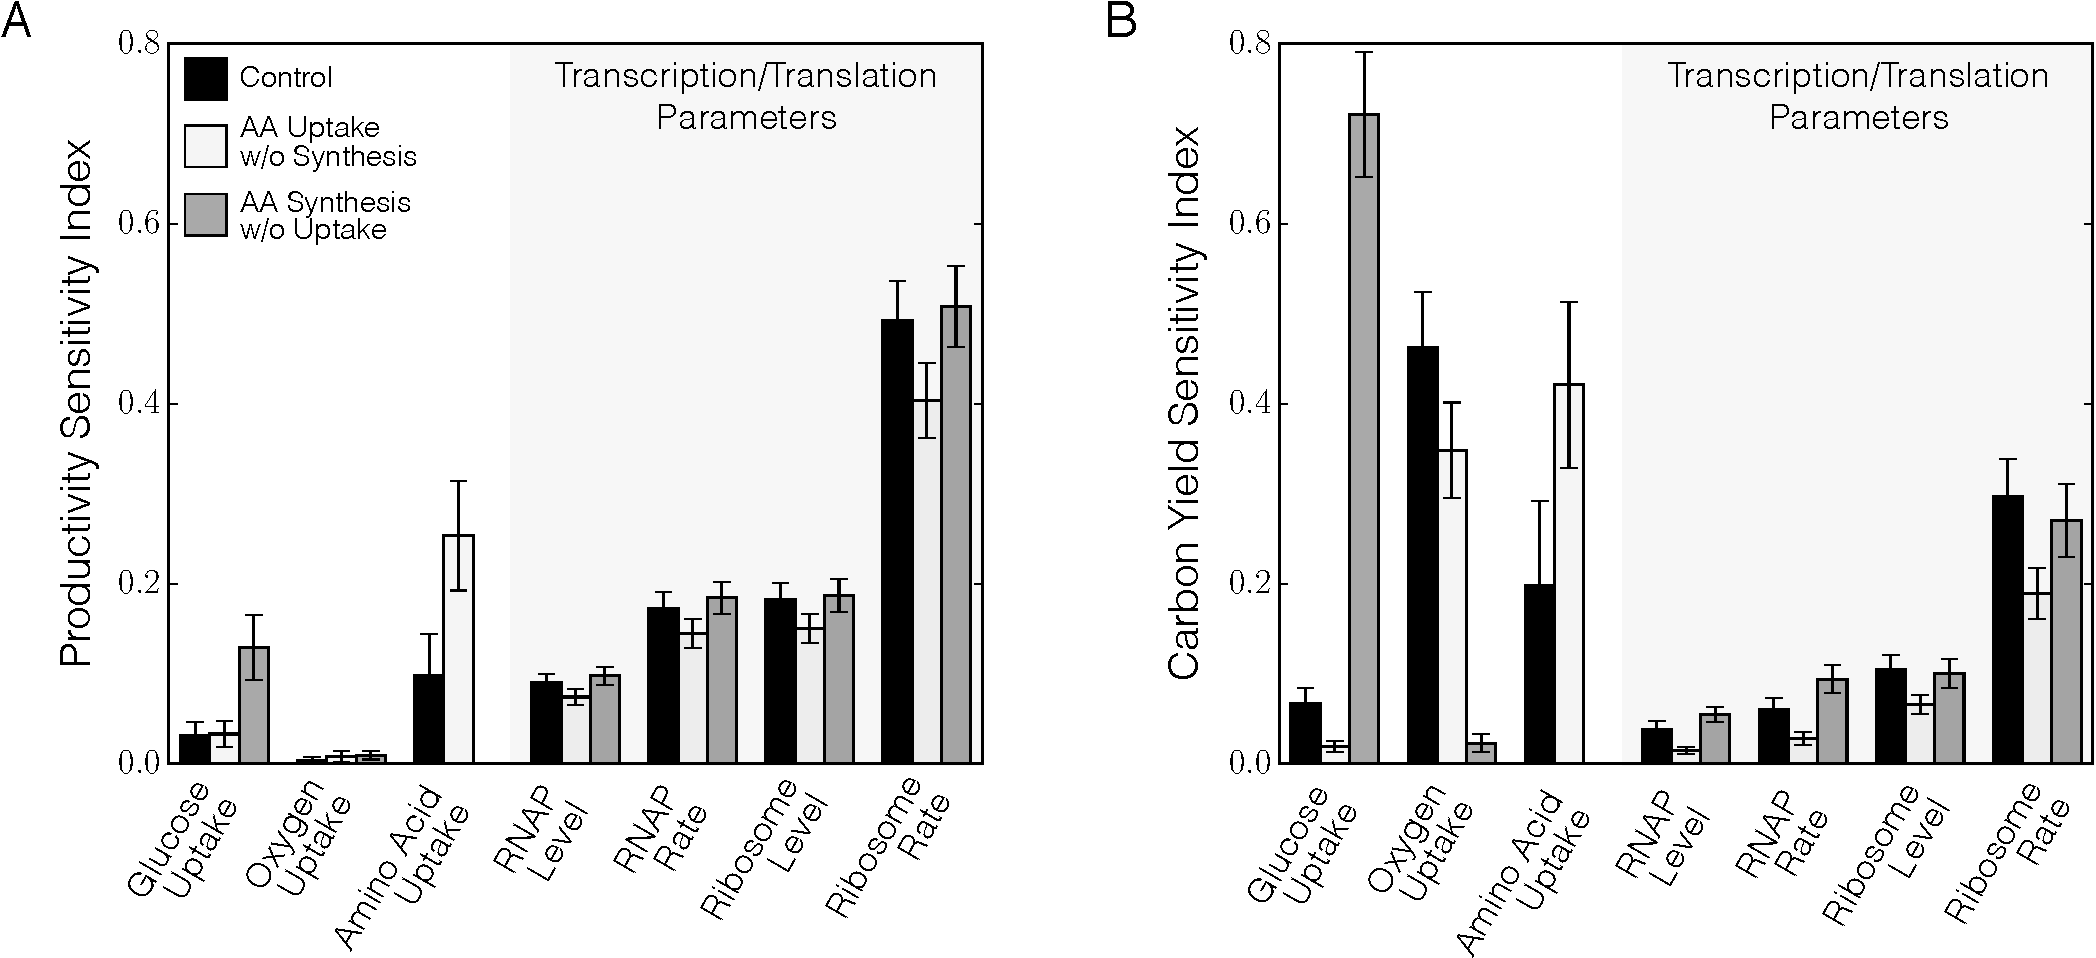
\includegraphics[width=1.00\textwidth]{./Figures/SI_GFP.pdf}
\caption{Total order sensitivity of deGFP productivity (A) and carbon yield (B) to specific uptake rates and transcription/translation parameters for three cases: control (black), amino acid uptake without synthesis (off white), and amino acid synthesis without uptake (gray). (Error bars represent 95\% CI of the ensemble).}
\label{fig:SI_GFP}
\end{figure}

When considering carbon yield performance (Fig \ref{fig:SI_GFP}B), the substrate and oxygen uptake fluxes became much more important while the sensitivity to the transcription/translation parameters decreased slightly.
The transcription/translation parameters had the same trend as for productivity, where the ribosome elongation rate was the most sensitive compared to the other transcription/translation parameters and showed significance across all parameters.
Thus, in investigating CFPS performance in terms of productivity and yield, the ribosome elongation rate is an important parameter to optimize, as been already shown in literature \cite{2005_underwood_biotech, 2014_li_PlosOne}.
Glucose and oxygen uptake shown significant importance for carbon yield since it determined the mechanism of energy generation, which is critical for efficient protein production.
Meanwhile, productivity is determined primarily by the rate of the most downstream steps, transcription and translation.
Glucose is required for both amino acid synthesis and efficient energy generation, both of which were important for a high yield.
There is a tradeoff between energy generation to power transcription/translation as well as the synthesis of amino acids which were required to assemble the protein of interest.
Across all three cases, substrate utilization (amino acid uptake and glucose) showed to be the next important as these substrates contributed to the carbon yield of deGFP.
Interestingly, in the first two cases, oxygen uptake had also a significant effect on carbon yield.
This is most likely due to the importance of oxidative phosphorylation for efficient energy generation.
With high oxidative phosphorylation, carbon substrates were not wasted to meet the necessary energy requirements of CFPS, instead the carbon was directed toward the production of deGFP.
However, in the third case (with no amino acid uptake), oxygen uptake significance decreased, while glucose uptake became the most siginificant.
When amino acids were not supplied in CFPS, glucose is the only carbon available for amino acid synthesis and energy generation. 
The same tradeoff was observed between utilizing glucose for amino acid synthesis and efficient energy generation; the significance of oxygen became irrelevant compared to the glucose uptake rate. 
In addition, NADH was required to power oxidative phosphorylation, however there was a higher demand for NADPH for amino acid syntheis since amino acids were required for the production of the protein of interest. 
Therefore, NADH was interconverted to NADPH, which decreased the significance of the oxygen uptake rate since there was not enough NADH to power oxidative phosphorylation.
Jewett and coworkers have reported that oxidative phosphorylation still operated in cell-free and also reported a decrease in yield, ranging from 1.5-fold to 4-fold, when oxidative phosphorylation reactions were knocked out\cite{Jewett:2008aa}.
However, it is unknown how active oxidative phosphorylation is compared to that of \textit{in vivo} systems, thus to investigate this further we compared deGFP carbon yield to oxidative phosphorylation flux (Fig \ref{fig:oxphos_yield}).
Interestingly, oxidative phosphorylation has a somewhat linear correlation with carbon yield for the first two cases (R\textsuperscript{2}=0.77 for the control, R\textsuperscript{2}=0.79 for the second case), whereas for the third case, this same effect was not as prevalent (R\textsuperscript{2}=0.46).
\begin{figure}[t!]
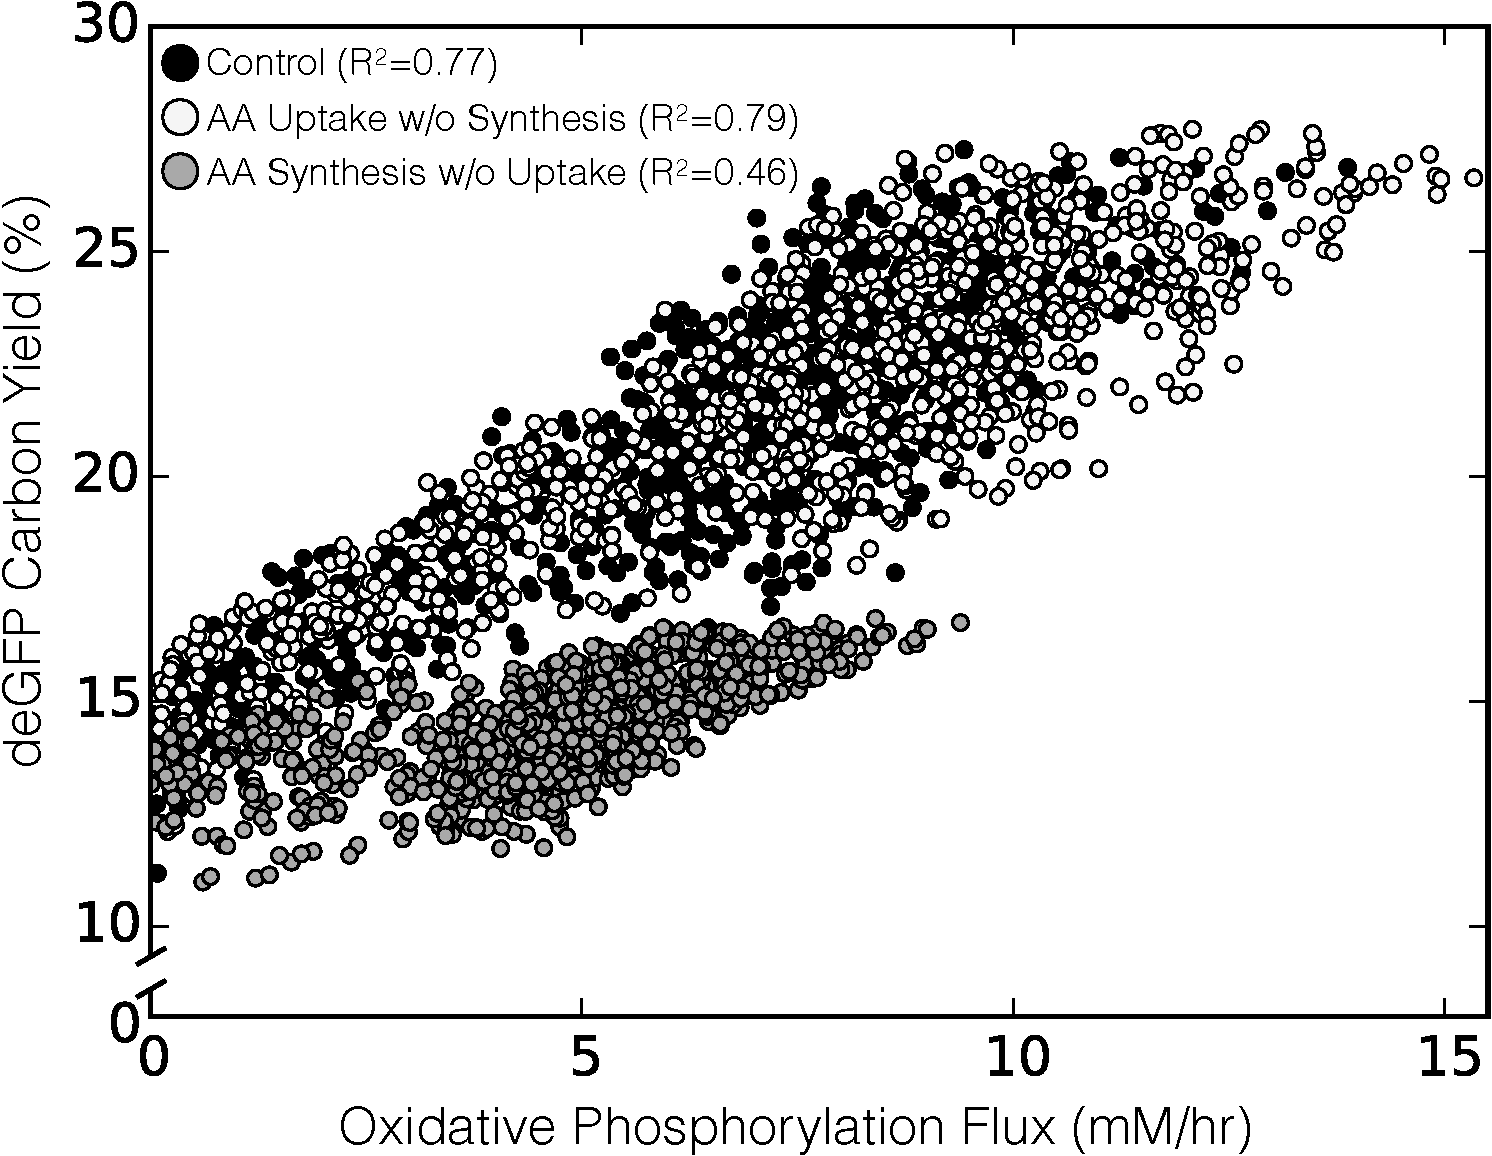
\includegraphics[width=0.7\textwidth]{./Figures/OxPhos_yield.pdf}
\caption{An ensemble of 1000 ssFBA solutions for deGFP carbon yield versus oxidative phosphorylation flux for three cases: control (black), amino acid uptake without synthesis (off white), and amino acid synthesis without uptake (gray). }
\label{fig:oxphos}
\end{figure}

When the system can utilize glucose for energy generation, the increase in oxidative phosphorylation has a positive effect on carbon yield.
However, when glucose is used to synthesize amino acids and power CFPS, there is a limit of how much oxidative phosphorylation can effect carbon yield due to the limitation of NADH to power oxidative phosphorylation.
Thus, it is interesting to see how much of the energetic needs of the system are met by oxidative phosphorylation and where the remaining energy is coming from.
To investigate the differences in productivity and carbon yields, we compared the flux distributions for deGFP predicted by ssFBA simulations for the three different cases (Fig.\ref{fig:flux}).
\begin{figure}[t!]
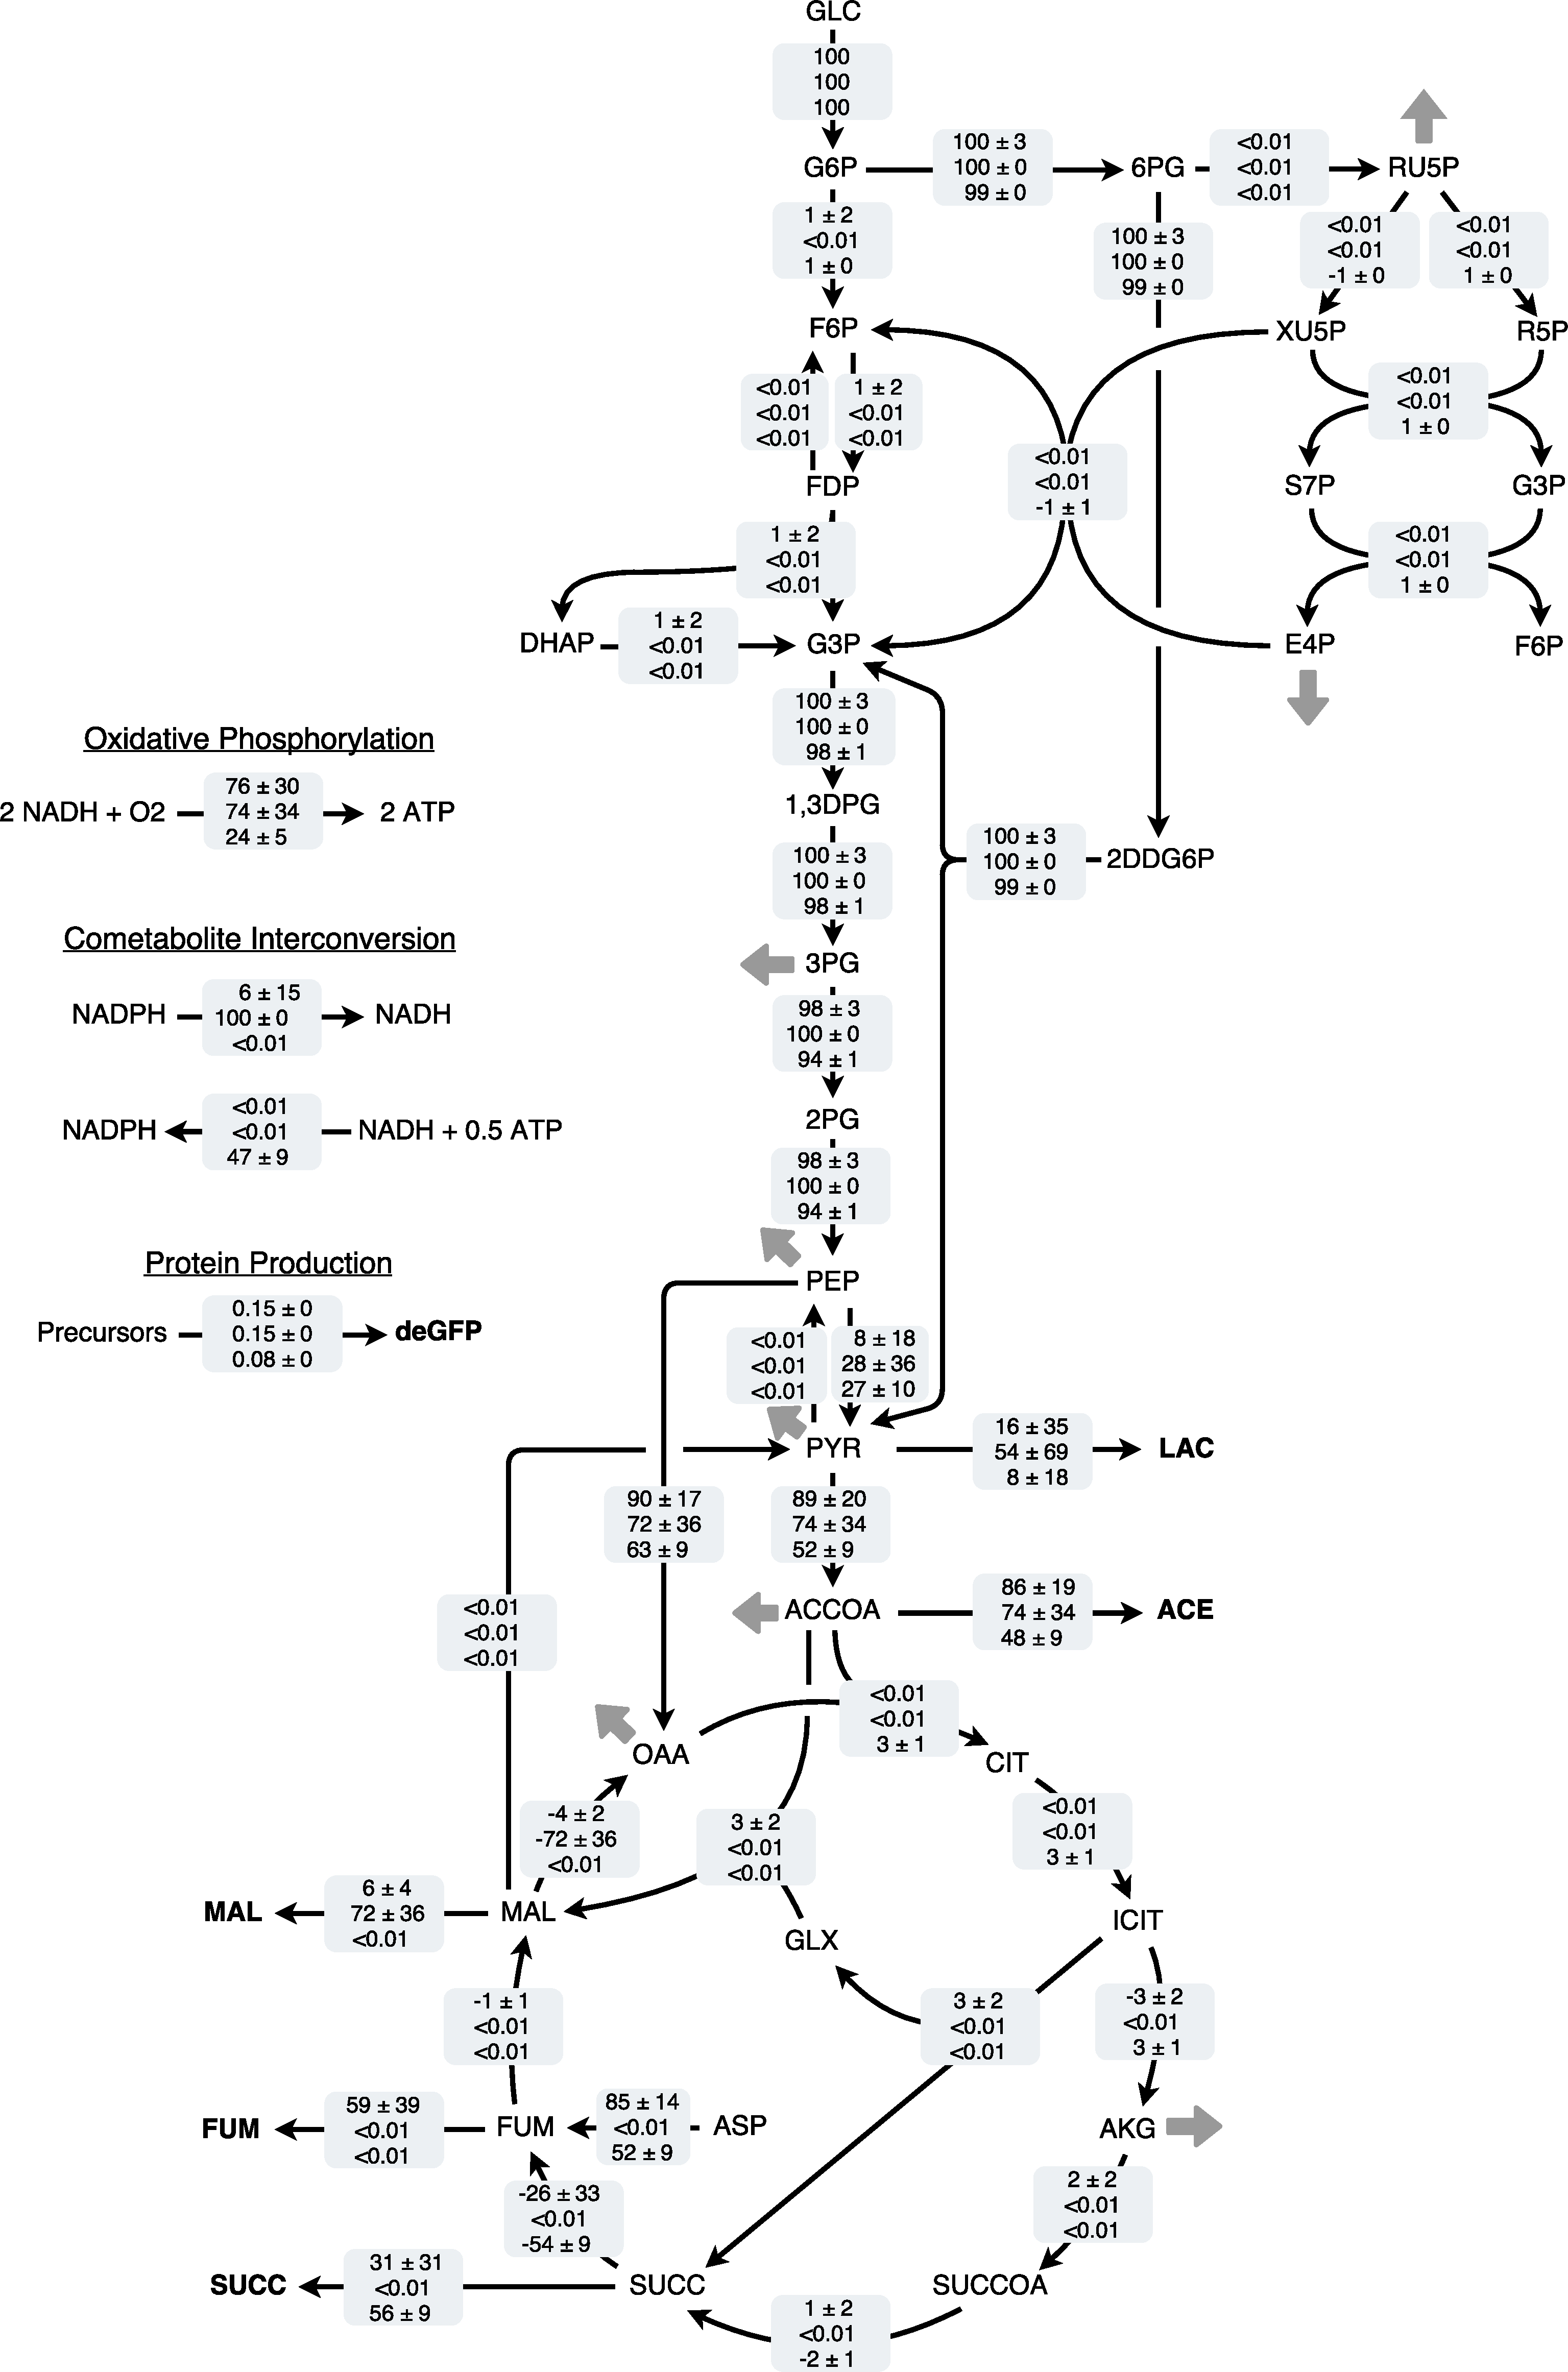
\includegraphics[width=0.78\textwidth]{./Figures/flux.pdf}
\caption{deGFP production flux profile for glycolysis, pentose phosphate pathway, Entner-Doudoroff pathway, TCA cycle, NADPH/NADH transfer, and oxidative phosphorylation. Flux (mean $\pm$ standard deviation) across ensemble normalized to glucose uptake flux. Flux distribution for three different cases: control (top row), amino acid uptake without synthesis (second row), and amino acid synthesis without uptake (third row). Bold metabolites are allowed to accumulate; grey arrows lead to amino acid synthesis.}
\label{fig:flux}
\end{figure}

All cases used the first step in the pentose phosphate pathway to generate NADPH;
the carbon flux then continued through the Entner–Doudoroff pathway toward pyruvate.
The majority of the flux was distributed between lactate and acetate, representing an inefficiency in energy generation as well as wasteful byproducts.
For the first two cases, the energy source was primarily oxidative phosphorylation, and to a lesser extent the TCA cycle.
The second case with no amino acid synthesis showed to be the most efficient process (highest carbon yield).
All the NADPH produced was interconverted to NADH to power oxidative phosphorylation.
Oxidative phosphorylation lead to a high redox ratio contributing to the accumulation of acetate overflow
However, diverting the flux away from acetate accumulation may allow more resources towards the protein of interest.
Interestingly, for the first case and more for the third case, there was a mixture of aerobic and anearobic energy generation.
Fumerate dehydrogenase typically operates in anaerobic conditions and was less efficient than oxidative phosphorylation.
Cell-free systems do not have a sense of regulation as \textit{in vivo} systems, thus any enzyme present in the mixture will carry out its corresponding reaction.
In the third case (third row), there was a low flux through oxidative phosphorylation and a high flux through fumerate dehydrogenase (fumerate to succinate).
One of the reasons for this inefficiency was some of the NADH is interconverted to NADPH which is required for amino acid synthesis, thus the lack of NADH cannot power oxidative phosphorylation as effectively as in the first two cases.
It is currently unknown how much oxidative phosphorylation is present in cell-free systems, however our model and the sensitivity analysis suggests that efficient energy generation is essential to higher carbon yields.
Thus, removing anaerobic enzymes during the cell-free extract preparation is a potential area for improvement for CFPS performance and protein yield.

All proteins followed a similar trend where for the first two cases (when amino acids were supplied) there was a relatively high yield than compared to the third case, with the exception of CAT.
Thus, we also performed a sensitivity analysis on CAT (Fig S1, available in the Supporting Information), which did not show the same trend in yield across the three cases as the other proteins.
For CAT, glucose uptake was as important to productivity as the kinetic parameters.
The oxygen uptake was the most important factor in yield and maintained this across all three cases.
The energy requirements for transcription of CAT is lower than the other proteins, thus it can accomodate its resources towards efficient energy generation.
Thus, the carbon yield was not hindered in the third case, since the system maintained the necessary amino acid synthesis rates and the required energy species.
Apart from these differences, there was a general trend of transcription and translation holding more significance for productivity and substrate uptake holding more significance for yield.

Taken together, we used sequence specific constraints based modeling to evaluate the performance of synthetic circuits in an \emph{E.~coli} cell-free protein synthesis (CFPS) system.
We have shown first principle predictions for protein production of deGFP and CAT under two different promoters and two different cell-free extract systems with no adjustable parameters were in agreement with experimental measurements.
This modeling approach validated general trends seen in literature for productivity and yield as a function of carbon number.
Further, global sensitivity analysis identified oxidative phosphorylation was instrumental for maintaining a high carbon yield and the translation rate was important for productivity.
The model also identified that cell-free systems can operate with aerobic and anaerobic enzymes which lead to inefficient CFPS systems and should be addressed to optimize carbon yield as seen in the globol sensitivity analysis.
In conclusion, sequence specific constraints based modeling offers a novel means to \emph{a~priori} estimate the performance of cell free synthetic circuits.


\section*{Materials and Methods}

\subsection*{Formulation and solution of the model equations.}
We estimated the theoretical maximum performance of the cell free protein synthesis system using sequence-specific flux balance analysis (ssFBA) \cite{Allen:2003aa}.
The sequence-specific flux balance analysis problem was formulated as a linear program:
\begin{equation}
 \begin{multlined}
	\qquad \qquad \qquad \max_{\boldsymbol{w}}{} \! \left( w_{TL} = \mathbf{\boldsymbol{\theta}}^T \boldsymbol{w} \right) \\
	\mathrm{Subject \; to:}
	 \; \; \mathbf{S}\mathbf{w}=\mathbf{0} \\
\alpha_i \leq w_i \leq \beta_i  \qquad i=1,2,\hdots,\mathcal{R}
 \end{multlined}
\end{equation}
where $\mathbf{S}$ denotes the stoichiometric matrix, $\mathbf{w}$ denotes the unknown flux vector, $\boldsymbol{\theta}$ denotes the objective selection vector
and $\alpha_i$ and $\beta_i$ denote the lower and upper bounds on flux $w_{i}$, respectively.
The stoichiometry of the kinetic model was used for the ssFBA calculations, with the execpetion of the transcription and translation rates.
The transcription (TX) and translation (TL) stoichiometry was modeled using the template reactions taken from Allen and Palsson \cite{Allen:2003aa}:
\begin{eqnarray*}
\mathrm{{G}_{\mathcal{P}}}+\mathrm{{R}_{1}} &\longrightarrow& \mathrm{G_{\mathcal{P}}^{*}} \\
\mathrm{G_{\mathcal{P}}^{*}}+\sum_{\mathrm{k\in\left\{A,C,G,U\right\}}}\eta_{k}\cdot \mathrm{\left\{k\right\}TP} &\overset{\rm TX}{\longrightarrow}& \mathrm{mRNA}+\mathrm{G_{\mathcal{P}}}+\mathrm{R_{1}}+ \mathrm{\sum_{k\in\left\{A,C,G,U\right\}}2\eta_{k}\cdot Pi}\\
\mathrm{mRNA} &\longrightarrow& \mathrm{\sum_{k\in\left\{A,C,G,U\right\}}\eta_{k}\cdot \left\{k\right\}MP} \\
\mathrm{mRNA}+\mathrm{R_{2}} &\longrightarrow& \mathrm{R_{2}^{*}} \\
\mathrm{\alpha_{j}\cdot AA_{j}+\alpha_{j}\cdot tRNA+\alpha_{j}\cdot ATP} &\longrightarrow& \mathrm{\alpha_{j}\cdot AA_{j}-tRNA_{j}+}\\
&& \mathrm{\qquad \alpha_{j}\cdot AMP+2\alpha_{j}\cdot Pi} \qquad{j=1,2,\hdots,20}\\
\mathrm{R_{2}^{*}+\sum_{j\in\left\{AA\right\}}\alpha_{j}\cdot \Big(AA_{j}-tRNA_{j}+2\cdot GTP\Big)} &\stackrel{\rm TL}{\longrightarrow}& \mathcal{P}+\mathrm{R_{2}+mRNA}+\\
&& \mathrm{\quad +\sum_{j\in\left\{AA\right\}}\alpha_{j}\cdot\Big(tRNA+2\cdot GDP+2\cdot Pi\Big)}
\end{eqnarray*}
where $G_{\mathcal{P}}$ denotes the gene encoding protein product $\mathcal{P}$,
$\rm R_{1}$ denotes the concentration of RNA polymerase,
$G_{\mathcal{P}}^{*}$ denotes the gene bounded by the RNA polymerase,
$\eta_{i}$ and $ \alpha_{j}$ denote the stoichiometric coefficients for nucleotide and amino acid, respectively,
$\rm Pi$ denotes inorganic phosphate,
$\rm R_{2}$ denotes the ribosome concentration,
$\rm R_{2}^{*}$ denotes bounded ribosome,
and $AA_{j}$ denotes $j^{th}$ amino acid.

The transcription rate ($w_{TX}$) was fixed in the ssFBA calculation at:
\begin{equation}
	w_{TX} = V_{TX}^{max}\left(\frac{G}{K_{TX}+G}\right)
\end{equation}
where $G$ denotes the gene concentration, and $K_{TX}$ denotes a transcription saturation coefficient.
The maximum rate of transcription $V_{TX}^{max}$ was formulated as:
\begin{equation}
	V_{TX}^{max} \equiv \left[R_{1}\left(\frac{v_{TX}}{l_{G}}\right)\mathcal{P}\right]
\end{equation}
The term $R_{1}$ denotes the RNA polymerase abundance,
$v_{TX}$ denotes the RNA polymerase elongation rate (nt/hr),
$l_{G}$ denotes the gene length in nucleotides, and the last term $\mathcal{P}$ describes a model of promoter activity.
In this study, we considered two promoters; the T7 and $\sigma_{70}$ promoters.
The promoter function for the T7 promoter, $\mathcal{P}_{T7}$ was given by:
\begin{equation}
	P_{T7} = (\frac{K_{T7}}{1 + K_{T7}}
\end{equation}
where $K_{T7}$ denotes a T7 RNA polymerase binding constant \cite{Moon:2012aa}.
The $\sigma_{70}$ binding promoter was used for all other proteins was formulated as:
\begin{equation}
	P_{\sigma_{70}} = \frac{K_{1}+K_{2}f_{p70}}{1 + K_{1}+K_{2}f_{p70}}
\end{equation}
where $K_{1}$ denotes the state of RNA polymerase binding,
$K_{2}$ is the state of $\sigma_{70} $binding along with RNA polymerase,
and $f_{p70}$ denotes the fraction of the $\sigma_{70}$ transcription factor bound to the promoter (modeled as a Hill function).

On the other hand, the translation rate ($w_{TL}$) was bounded by:
 \begin{equation}
	0\leq w_{TL} \leq V_{TL}^{max}\left(\frac{\rm mRNA_{SS}}{K_{TL}+\rm mRNA_{SS}}\right)
\end{equation}
where $\rm mRNA_{SS}$ denotes the steady state mRNA abundance, and $K_{TL}$ denotes the translation saturation constant.
The maximum translation rate $V_{TL}^{max}$ was formulated as:
\begin{equation}
	V_{TL}^{max} \equiv \left[K_{P} R_{2}\left(\frac{v_{TL}}{l_{P}}\right)\right]
\end{equation}
The term $K_{P}$ denotes the polysome amplification constant,
$v_{TL}$ denotes the ribosome elongation rate (amino acids per hour),
$l_{P}$ denotes the number of amino acids in the protein of interest,
and $\rm mRNA_{SS}$ denotes the steady-state mRNA concentration:
\begin{equation}
	\rm mRNA_{SS}\simeq\frac{w_{TX}}{\lambda}
\end{equation}where $\lambda$ denotes the rate constant controlling the mRNA degradation rate.

The objective of the sequence-specific flux balance calculation was to maximize the rate of protein translation, $w_{TL}$.
The total glucose uptake rate was bounded by [0,40 mM/h] according to experimental data;
while the amino acid uptake rates were bounded by [0,30 mM/h], but did not reach the maximum flux.
The protein gene and protein sequences were taken from literature and are available in the Supporting Information.
The sequence-specific flux balance linear program was solved using the GNU Linear Programming Kit (GLPK) v4.52 \cite{GLPK}.

% The flux balance analysis problem was formulated as:
% \begin{equation}\nonumber
%  \begin{multlined}
% 	\qquad \qquad \qquad \max_{\boldsymbol{w}}{} \! \left( w_{obj} = \mathbf{\boldsymbol{\theta}}^T \boldsymbol{w} \right) \\
% 	\mathrm{Subject \; to:}
% 	 \; \; \mathbf{S}\mathbf{w}=\mathbf{0} \\
% \alpha_i \leq w_i \leq \beta_i  \qquad i=1,2,\hdots,\mathcal{R}
%  \end{multlined}
% \end{equation}
% where $\mathbf{S}$ denotes the stoichiometric matrix, $\mathbf{w}$ denotes the unknown flux vector, $\boldsymbol{\theta}$ denotes the objective selection vector
% and $\alpha_i$ and $\beta_i$ denote the lower and upper bounds on flux $w_{i}$, respectively.
% The flux balance analysis problem was solved using the GNU Linear Programming Kit (v4.52) \cite{GLPK}.
%
% \subsection*{Sequence-specific flux balance analysis}
% We estimated the theoretical maximum carbon yield using sequence-specific flux balance analysis (ssFBA) \cite{Allen:2003aa}.
% The sequence-specific flux balance analysis problem was formulated as a linear program:
% \begin{equation}
%  \begin{multlined}
% 	\qquad \qquad \qquad \max_{\boldsymbol{w}}{} \! \left( w_{TL} = \mathbf{\boldsymbol{\theta}}^T \boldsymbol{w} \right) \\
% 	\mathrm{Subject \; to:}
% 	 \; \; \mathbf{S}\mathbf{w}=\mathbf{0} \\
% \alpha_i \leq w_i \leq \beta_i  \qquad i=1,2,\hdots,\mathcal{R}
%  \end{multlined}
% \end{equation}
% where $\mathbf{S}$ denotes the stoichiometric matrix, $\mathbf{w}$ denotes the unknown flux vector, $\boldsymbol{\theta}$ denotes the objective selection vector
% and $\alpha_i$ and $\beta_i$ denote the lower and upper bounds on flux $w_{i}$, respectively.
% The stoichiometry of the kinetic model was used for the ssFBA calculations, with the execpetion of the transcription and translation rates.
% The transcription (TX) and translation (TL) stoichiometry was modeled using the template reactions taken from Allen and Palsson \cite{Allen:2003aa}:
% \begin{eqnarray*}
% \mathrm{{G}_{\mathcal{P}}}+\mathrm{{R}_{1}} &\longrightarrow& \mathrm{G_{\mathcal{P}}^{*}} \\
% \mathrm{G_{\mathcal{P}}^{*}}+\sum_{\mathrm{k\in\left\{A,C,G,U\right\}}}\eta_{k}\cdot \mathrm{\left\{k\right\}TP} &\overset{\rm TX}{\longrightarrow}& \mathrm{mRNA}+\mathrm{G_{\mathcal{P}}}+\mathrm{R_{1}}+ \mathrm{\sum_{k\in\left\{A,C,G,U\right\}}2\eta_{k}\cdot Pi}\\
% \mathrm{mRNA} &\longrightarrow& \mathrm{\sum_{k\in\left\{A,C,G,U\right\}}\eta_{k}\cdot \left\{k\right\}MP} \\
% \mathrm{mRNA}+\mathrm{R_{2}} &\longrightarrow& \mathrm{R_{2}^{*}} \\
% \mathrm{\alpha_{j}\cdot AA_{j}+\alpha_{j}\cdot tRNA+\alpha_{j}\cdot ATP} &\longrightarrow& \mathrm{\alpha_{j}\cdot AA_{j}-tRNA_{j}+}\\
% && \mathrm{\qquad \alpha_{j}\cdot AMP+2\alpha_{j}\cdot Pi} \qquad{j=1,2,\hdots,20}\\
% \mathrm{R_{2}^{*}+\sum_{j\in\left\{AA\right\}}\alpha_{j}\cdot \Big(AA_{j}-tRNA_{j}+2\cdot GTP\Big)} &\stackrel{\rm TL}{\longrightarrow}& \mathcal{P}+\mathrm{R_{2}+mRNA}+\\
% && \mathrm{\quad +\sum_{j\in\left\{AA\right\}}\alpha_{j}\cdot\Big(tRNA+2\cdot GDP+2\cdot Pi\Big)}
% \end{eqnarray*}
% where $G_{\mathcal{P}}$ denotes the gene encoding protein product $\mathcal{P}$,
% $\rm R_{1}$ denotes the concentration of RNA polymerase,
% $G_{\mathcal{P}}^{*}$ denotes the gene bounded by the RNA polymerase,
% $\eta_{i}$ and $ \alpha_{j}$ denote the stoichiometric coefficients for nucleotide and amino acid, respectively,
% $\rm Pi$ denotes inorganic phosphate,
% $\rm R_{2}$ denotes the ribosome concentration,
% $\rm R_{2}^{*}$ denotes bounded ribosome,
% and $AA_{j}$ denotes $j^{th}$ amino acid.
%
% The transcription rate ($w_{TX}$) was fixed in the ssFBA calculation at:
% \begin{equation}
% 	w_{TX} = V_{TX}^{max}\left(\frac{G}{K_{TX}+G}\right)
% \end{equation}
% where $G$ denotes the gene concentration, and $K_{TX}$ denotes a transcription saturation coefficient.
% The maximum rate of transcription $V_{TX}^{max}$ was formulated as:
% \begin{equation}
% 	V_{TX}^{max} \equiv \left[R_{1}\left(\frac{v_{TX}}{l_{G}}\right)P\right]
% \end{equation}
% The term $R_{1}$ denotes the RNA polymerase abundance,
% $v_{TX}$ denotes the RNA polymerase elongation rate (nt/hr),
% $l_{G}$ denotes the gene length in nucleotides, and $P$ describes the promoter activity.
%  The T7 binding promoter was used for CAT production was formulated as:
%
%
% On the other hand, the translation rate ($w_{TL}$) was bounded by:
%  \begin{equation}
% 	0\leq w_{TL} \leq V_{TL}^{max}\left(\frac{\rm mRNA_{SS}}{K_{TL}+\rm mRNA_{SS}}\right)
% \end{equation}
% where $\rm mRNA_{SS}$ denotes the steady state mRNA abundance, and $K_{TL}$ denotes the translation saturation constant.
% The maximum translation rate $V_{TL}^{max}$ was formulated as:
% \begin{equation}
% 	V_{TL}^{max} \equiv \left[K_{P} R_{2}\left(\frac{v_{TL}}{l_{P}}\right)\right]
% \end{equation}
% The term $K_{P}$ denotes the polysome amplification constant,
% $v_{TL}$ denotes the ribosome elongation rate (amino acids per hour),
% $l_{P}$ denotes the number of amino acids in the protein of interest,
% and $\rm mRNA_{SS}$ denotes the steady-state mRNA concentration:
% \begin{equation}
% 	\rm mRNA_{SS}\simeq\frac{w_{TX}}{\lambda}
% \end{equation}where $\lambda$ denotes the rate constant controlling the mRNA degradation rate.
%
% The objective of the sequence-specific flux balance calculation was to maximize the rate of CAT translation, $w_{TL}$.
% The total glucose uptake rate was bounded by [0,40 mM/h] according to experimental data;
% while the amino acid uptake rates were bounded by [0,30 mM/h], but did not reach the maximum flux.
% The protein gene and protein sequences were taken from literature and are available in the Supporting Information.
% The sequence-specific flux balance linear program was solved using the GNU Linear Programming Kit (GLPK) v4.52 \cite{GLPK}.

\subsection*{Calculation of the carbon yield.}
The carbon yield ($Y_{C}^{POI}$) was calculated as the ratio of carbon produced as the protein of interest divided by the carbon consumed as reactants (glucose and amino acids):
\begin{equation}\label{eqn:yield-definition}
	Y_{C}^{POI}=\frac{\Delta\texttt{POI}\cdot C_{POI}}{\displaystyle\sum_{i=1}^{\mathcal{R}}\max(\Delta m_{i},0)\cdot C_{m_i}}
\end{equation}
where $\Delta\texttt{POI}$ denotes the abundance of the protein of interest produced, $C_{POI}$ denotes carbon number of the protein of interest, $\mathcal{R}$ denotes the number of reactants,
$\Delta m_{i}$ denotes the amount of the $i^{th}$ reactant consumed (never allowed to be negative), and $C_{m_i}$ denotes the carbon number of the $i^{th}$ reactant.

\subsubsection*{Quantification of uncertainty.}
An ensemble of 100 sets of flux distributions was calculated for three different cases: control (with amino acid synthesis and uptake), amino acid uptake without synthesis, and amino acid synthesis without uptake.
An ensemble of flux distributions was then calculated by randomly sampling the maximum specific glucose uptake rate from within a range of 30 to 40 mM/h, determined from experimental data and randomly sampling oxygen uptake, RNAP polymerase levels, ribosome levels, and elongation rates in a physiological range determined from literature.
RNA polymerase levels were sampled between 60 and 80 nM, ribosome levels between 7 and 16 \textmu M, the RNA polymerase elongation rate between 20 and 30 nt/sec, and the ribosome elongation rate between 1.5 and 3 aa/sec \cite{2005_underwood_biotech, Garamella:2016aa}.

\subsection*{Global sensitivity analysis.}
We conducted a global sensitivity analysis, using the variance-based method of Sobol, to estimate which parameters controlled the performance of synthetic circuits \citep{SOBOL_METHOD}.
We computed the total sensitivity index of each parameter relative to two performance objectives, productivity of the protein of interest and the carbon yield.
We established the sampling bounds for each parameter from literature.
We used the sampling method of Saltelli \textit{et al.} \citep{Saltelli:2010} to compute a family of $N\left(2d+2\right)$ parameter sets which obeyed our parameter ranges,
where $N$ was the number of trials, and $d$ was the number of parameters in the model. In our case, $N$ = 1,000 and $d$ = 7, so the total sensitivity indices were computed from
16,000 model evaluations. The variance-based sensitivity analysis was conducted using the SALib module encoded in the Python programming language \citep{SALIB}.

%%%%%%%%%%%%%%%%%%%%%%%%%%%%%%%%%%%%%%%%%%%%%%%%%%%%%%%%%%%%%%%%%%%%%
%% The "Acknowledgement" section can be given in all manuscript
%% classes.  This should be given within the "acknowledgement"
%% environment, which will make the correct section or running title.
%%%%%%%%%%%%%%%%%%%%%%%%%%%%%%%%%%%%%%%%%%%%%%%%%%%%%%%%%%%%%%%%%%%%%
\begin{acknowledgement}

Please use ``The authors thank \ldots'' rather than ``The
authors would like to thank \ldots''.

The author thanks Mats Dahlgren for version one of \textsf{achemso},
and Donald Arseneau for the code taken from \textsf{cite} to move
citations after punctuation. Many users have provided feedback on the
class, which is reflected in all of the different demonstrations
shown in this document.

\end{acknowledgement}

%%%%%%%%%%%%%%%%%%%%%%%%%%%%%%%%%%%%%%%%%%%%%%%%%%%%%%%%%%%%%%%%%%%%%
%% The same is true for Supporting Information, which should use the
%% suppinfo environment.
%%%%%%%%%%%%%%%%%%%%%%%%%%%%%%%%%%%%%%%%%%%%%%%%%%%%%%%%%%%%%%%%%%%%%
\begin{suppinfo}

The following files are available free of charge.
\begin{itemize}
  \item Protein Sequences: DNA and protein sequences of each protein of interest.
  \item CAT Sensitivity: Global sensitivity analysis of CAT productivity and carbon yield.
\end{itemize}

\end{suppinfo}

%%%%%%%%%%%%%%%%%%%%%%%%%%%%%%%%%%%%%%%%%%%%%%%%%%%%%%%%%%%%%%%%%%%%%
%% The appropriate \bibliography command should be placed here.
%% Notice that the class file automatically sets \bibliographystyle
%% and also names the section correctly.
%%%%%%%%%%%%%%%%%%%%%%%%%%%%%%%%%%%%%%%%%%%%%%%%%%%%%%%%%%%%%%%%%%%%%
\bibliography{References_v1}

\end{document}
